\documentclass[aps,prd,preprint,nofootinbib,superscriptaddress]{revtex4-2}

\usepackage{amsmath,amssymb,bm}
\usepackage{graphicx}
\usepackage{booktabs}
\usepackage{hyperref}
\providecommand{\FloatBarrier}{\clearpage}
\usepackage{xcolor}

\begin{document}

\title{A Phenomenological Bound-Domain Response Law for SPARC Flat Velocities}

\author{Author names withheld for draft review}
\affiliation{Affiliations withheld for draft review}

\date{\today}

\begin{abstract}
We present a phenomenological effective law for flat rotation velocities in disk galaxies. The model, which we denote bound-domain vacuum response (BDVR), augments the baryonic acceleration with a low-acceleration term whose amplitude depends on a global normalization and on radial, gas-content, and morphology modifiers. We evaluate a frozen parameter realization on an 87-galaxy SPARC quality-1 subset with positive $V_{\mathrm{flat}}$, $L_{3.6}$, $M_{\mathrm{H\,I}}$, and $R_d$, using no per-galaxy parameter adjustment and no removal of high-residual objects. On this restricted sample, the model yields a median absolute residual of 0.0416 dex in $\log_{10}(V_{\mathrm{pred}}/V_{\mathrm{obs}})$, compared with 0.0472 dex for a simple BTFR-like baseline. These results show that the frozen parameterization is competitive as a restricted predictor of $V_{\mathrm{flat}}$ on this sample, but they do not establish a derived theory, a cosmological framework, or a dark-matter replacement. The current analysis omits full rotation-curve fitting, observational uncertainty propagation, and formal model comparison; it also does not test lensing, clustering, or cosmological constraints. We therefore treat BDVR as a falsifiable phenomenological ansatz whose status depends on those next tests.
\end{abstract}

\maketitle

\section{Introduction}

Disk-galaxy rotation speeds obey tight empirical relations with their baryonic mass distribution, most prominently the baryonic Tully--Fisher relation (BTFR) and the radial acceleration relation (RAR). These relations are now studied routinely with the SPARC database, which combines near-infrared photometry with high-quality H~I/H$\alpha$ rotation curves across a wide range of galaxy masses, surface brightnesses, and gas fractions. Any new effective law for galaxy rotation phenomenology should therefore be tested against SPARC and compared directly with BTFR-, RAR-, and halo-based baselines.

In this paper we do not attempt a full theory of galaxy dynamics. Instead, we test whether a frozen phenomenological response law, motivated by a broader measurement-domain framework, can predict the flat rotation velocity $V_{\rm flat}$ from baryonic quantities without per-galaxy parameter adjustment. The goal is not to replace dark matter or to fit full rotation curves, but to determine whether the proposed radial and structural modifiers provide statistically meaningful predictive power beyond simpler baryonic scalings.

The Hubble-tension ancestry is not used as evidence in this galaxy-sector test. It appears only as historical motivation for separating local calibration or bound-domain effects from extended photon-propagation effects. Because the present paper tests only a galaxy-sector $V_{\rm flat}$ relation, all cosmological ancestry is treated as historical motivation rather than evidence; the empirical burden of the paper lies entirely in its SPARC benchmark.

\section{Parent CGHSTC measurement-domain formulation}

CGHSTC-34 assigns an observable to a measurement domain
\begin{equation}
M = (\mathcal{B},\mathcal{N},\mathcal{D},\mathcal{E},\mathcal{T}),
\end{equation}
where $\mathcal{B}$ denotes bound/coherent structure, $\mathcal{N}$ null-path extent, $\mathcal{D}$ decoherence or path averaging, $\mathcal{E}$ environmental or potential coupling, and $\mathcal{T}$ the operational clock or calibration character of the measurement.

The first-pass domain functional is
\begin{equation}
Q(M)=\sigma\!\left[
 a_B\mathcal{B}(M)
-a_N\mathcal{N}(M)
-a_D\mathcal{D}(M)
+a_E\mathcal{E}(M)-b
\right],
\qquad
\sigma(x)=\frac{1}{1+e^{-x}} .
\end{equation}
Thus $Q(M)$ is large for active bound domains and small for extended null or strongly averaged domains. The associated clock-current factor is written
\begin{equation}
\Gamma(M)=1-\epsilon_0 Q(M).
\end{equation}

For a local calibration domain one may write
\begin{equation}
H_{0,\rm local}=\frac{H_{0,\rm cos}}{\Gamma_{\rm cal,0}}.
\end{equation}
Using the inherited reference values $H_{0,\rm cos}=67.4\,{\rm km\,s^{-1}\,Mpc^{-1}}$ and $H_{0,\rm local}=73.04\,{\rm km\,s^{-1}\,Mpc^{-1}}$ gives $\Gamma_{\rm cal,0}\simeq0.92278$ and $\epsilon_0\simeq0.07722$ for a strongly coupled calibration domain. This calibration relation is used here only as scale-setting context and ancestry for the sector separation; the present manuscript does not claim a Hubble-tension solution.

For an extended propagation domain, $Q(M_{\rm prop})\ll1$, so
\begin{equation}
\Gamma_{\rm prop}(M)=1-\epsilon_0 Q(M)\simeq1.
\end{equation}
A simple propagation-suppression estimate is
\begin{equation}
\left|\frac{\Delta D}{D}\right|\lesssim \epsilon_0 Q_{\rm prop,max} .
\end{equation}
This is the mathematical transition to BDVR: a galaxy rotation measurement is a bound-domain observable with $Q(M_{\rm gal})$ not forced to vanish, whereas SN, BAO, and CMB distance propagation can remain in a suppressed-coupling domain. In the present paper, Eq.~(2) is used only as a heuristic motivation for a galaxy-sector parameterization; we do not derive Eqs.~(8)--(13) from Eq.~(2).

\section{BDVR galaxy-sector effective law}

BDVR is the galaxy-sector effective law produced by resolving the active bound-galaxy response into radial and structural factors. The radial diagnostic acceleration form is
\begin{equation}
a_{\rm obs}(r) = a_b(r) + a_{\rm BDVR}(r),
\end{equation}
with
\begin{equation}
a_{\rm BDVR}(r) = Q_{\rm eff}(r,g)\sqrt{a_b(r)a_0} .
\end{equation}
Here $a_b(r)$ is the baryonic Newtonian acceleration and $a_0=1.2\times10^{-10}\,{\rm m\,s^{-2}}$ is the reference acceleration scale used in the frozen evaluation.

The operational galaxy-sector response factor is
\begin{equation}
Q_{\rm eff}(r,g) = Q_0 H(r/R_d) S_{\rm sg}(g) S_{\rm int}(g).
\end{equation}
The radial halo activation is
\begin{equation}
H(r/R_d) = 1 + A_h \left[1 - \exp\left(-\frac{r}{k_h R_d}\right)\right].
\end{equation}
The stellar/gas structural factor is
\begin{equation}
S_{\rm sg} =
1 + A_{\rm sg}\max\left[0,\log_{10}\left(\frac{M_*}{M_g}\right)-\log_{10}(5)\right].
\end{equation}
The internal morphology factor is
\begin{equation}
S_{\rm int} = 1 + A_{\rm int}\max(0,5-T_{\mathrm{morph}}).
\end{equation}

For SPARC Table-1 flat-velocity comparisons we use
\begin{equation}
v_{\rm flat}^{\rm BDVR} =
\left(Q_{\rm eff}^2 G M_{\mathrm{bar}} a_0\right)^{1/4} .
\end{equation}
This is a restricted $V_{\rm flat}$ estimator, not a full rotation-curve solution. The adaptive radius enters only through $Q_{\rm eff}$. The SPARC flat-velocity comparison is not computed as $\sqrt{r a_{\rm total}}$, and the present evaluation is not a full rotation-curve fit. Because the flat-velocity estimator has the same $V^4\propto G M_{\rm bar} a_0$ scaling as BTFR-like laws up to a multiplicative factor $Q_{\rm eff}^2$, the critical methodological question is whether the added radial and structural modifiers improve predictive performance under uncertainty-aware comparison to simpler baselines.

\section{Frozen parameter set}

\begin{table*}[t]
\centering
\scriptsize
\caption{Frozen parameters used in the M4c/M5 BDVR frozen-run benchmark. All values are global and are not adjusted per galaxy.}
\label{tab:frozen-parameters}
\resizebox{\textwidth}{!}{%
\begin{tabular}{lll}
\toprule
Parameter & Value & Description \\
\midrule
$Q_0$ & 0.9002495108803148 & Global baseline BDVR galaxy-sector response amplitude \\
$a_0$ (m s$^{-2}$) & 1.2e-10 & Reference acceleration scale \\
$A_h$ & 0.35 & Amplitude of radial halo activation \\
$k_h$ & 3.0 & Halo scale length in units of Rdisk \\
$r_{\mathrm{eval}}$ mode & transition & Adaptive radius mode used to evaluate $Q_{\mathrm{eff}}$ \\
velocity mode & flat\_response & Flat-response estimator for SPARC Table-1 $V_{\mathrm{flat}}$ \\
fallback $r_{\mathrm{eval}}/R_d$ & 4.0 & Fallback $r_{\mathrm{eval}}/R_d$ \\
min $r_{\mathrm{eval}}/R_d$ & 1.5 & Minimum clipped $r_{\mathrm{eval}}/R_d$ \\
max $r_{\mathrm{eval}}/R_d$ & 12.0 & Maximum clipped $r_{\mathrm{eval}}/R_d$ \\
$S_{\mathrm{sg}}$ mode & star\_gas\_hinge & Star/gas structural response mode \\
$A_{\mathrm{sg}}$ & 0.3 & Star/gas hinge amplitude \\
$M_*/M_g$ hinge threshold & 5.0 & Threshold for stellar-to-gas ratio hinge \\
$S_{\mathrm{int}}$ mode & early\_type\_hinge & Internal morphology response mode \\
$A_{\mathrm{int}}$ & 0.1 & Early-type morphology hinge amplitude \\
$T_{\mathrm{morph}}$ threshold & 5.0 & Morphological $T_{\mathrm{morph}}$ threshold for early-type response \\
\bottomrule
\end{tabular}%
}
\end{table*}

All parameters in Table~\ref{tab:frozen-parameters} are global. They are not adjusted per galaxy in the evaluation subset. As a frozen-parameter provenance note, the available artifact record does not yet provide a complete training, tuning, and validation chronology for every global design choice. The current text therefore treats the frozen status as a reproducibility constraint on this run, not as proof that the evaluation subset never informed earlier model design.

\section{Data and evaluation protocol}

The evaluation uses a SPARC quality-1 sample with positive $V_{\rm flat}$, $L_{3.6}$, $M_{\rm H\,I}$, and $R_d$. The frozen model is evaluated with no per-galaxy response adjustment, no retuning on the evaluation subset, and no deletion of the leading residual object. The exact 87-galaxy evaluation table, M4c residual vector, ablation residual vectors, and freeze-chronology status table are included as machine-readable CSV files in the generated \texttt{tables/} directory.

The stellar and gas masses are constructed as
\begin{equation}
M_* = 0.5 L_{3.6} \times 10^9 M_\odot,
\end{equation}
and
\begin{equation}
M_g = 1.33 M_{\rm H\,I} \times 10^9 M_\odot.
\end{equation}
Unless otherwise stated, $M_{\mathrm{bar}} \equiv M_* + M_g$. The ordered evaluation-radius algorithm is: (i) if a transition radius is recorded in the frozen input table, read that value; (ii) express it in units of the disk scale length as $r/R_d$; (iii) clip the value to $1.5\le r_{\mathrm{eval}}/R_d\le12$ so that extremely small or pathological radii do not dominate the flat-velocity estimator; and (iv) otherwise set $r_{\mathrm{eval}}=4R_d$. The resulting value is stored as \texttt{r\_over\_Rdisk\_eval} in the complete machine-readable 87-galaxy table.

The residual for galaxy $i$ is
\begin{equation}
\Delta_i=\log_{10}V_{{\rm pred},i}-\log_{10}V_{{\rm obs},i}.
\end{equation}
A formal next-stage comparison should use a likelihood such as
\begin{equation}
\ln \mathcal{L}=-\frac{1}{2}\sum_i\left[\frac{\Delta_i^2}{\sigma_i^2}+\ln(2\pi\sigma_i^2)\right],
\end{equation}
where $\sigma_i^2$ would include observational variance in $V_{\rm flat}$ plus propagated distance, inclination, stellar mass-to-light, H I mass, and intrinsic-scatter terms. At present, observational uncertainties are not propagated in the current artifact set; confidence intervals, bootstrap resampling, and likelihood-level covariance treatment remain required before the residual differences can be treated as decisive model-selection evidence. The limitation can be summarized directly: observational uncertainties are not propagated in the current artifact set.

\section{Frozen M4c evaluation result}

\begin{table*}[t]
\centering
\scriptsize
\caption{Frozen M4c evaluation summary for the SPARC quality-1 flat-velocity sample.}
\label{tab:m5-summary}
\resizebox{\textwidth}{!}{%
\begin{tabular}{lll}
\toprule
Metric & Value & Description \\
\midrule
n\_galaxies & 87 & SPARC quality-1 galaxies in frozen M5 validation \\
median\_abs\_log10\_velocity\_error & 0.041613899469354995 & Median absolute log10(pred/obs) \\
mean\_abs\_log10\_velocity\_error & 0.04572143797277067 & Mean absolute log10(pred/obs) \\
max\_abs\_log10\_velocity\_error & 0.23214012979801618 & Maximum absolute log10(pred/obs) \\
median\_velocity\_ratio\_pred\_over\_obs & 1.0215021046046753 & Median predicted/observed velocity ratio \\
frac\_within\_010\_dex & 0.9540229885057471 & Fraction within 0.10 dex \\
frac\_within\_015\_dex & 0.9885057471264368 & Fraction within 0.15 dex \\
frac\_within\_020\_dex & 0.9885057471264368 & Fraction within 0.20 dex \\
n\_within\_010\_dex & 83 & Count within 0.10 dex \\
n\_within\_015\_dex & 86 & Count within 0.15 dex \\
n\_within\_020\_dex & 86 & Count within 0.20 dex \\
n\_above\_030\_dex & 0 & Count above 0.30 dex \\
\bottomrule
\end{tabular}%
}
\end{table*}

\begin{figure*}[t]
\centering
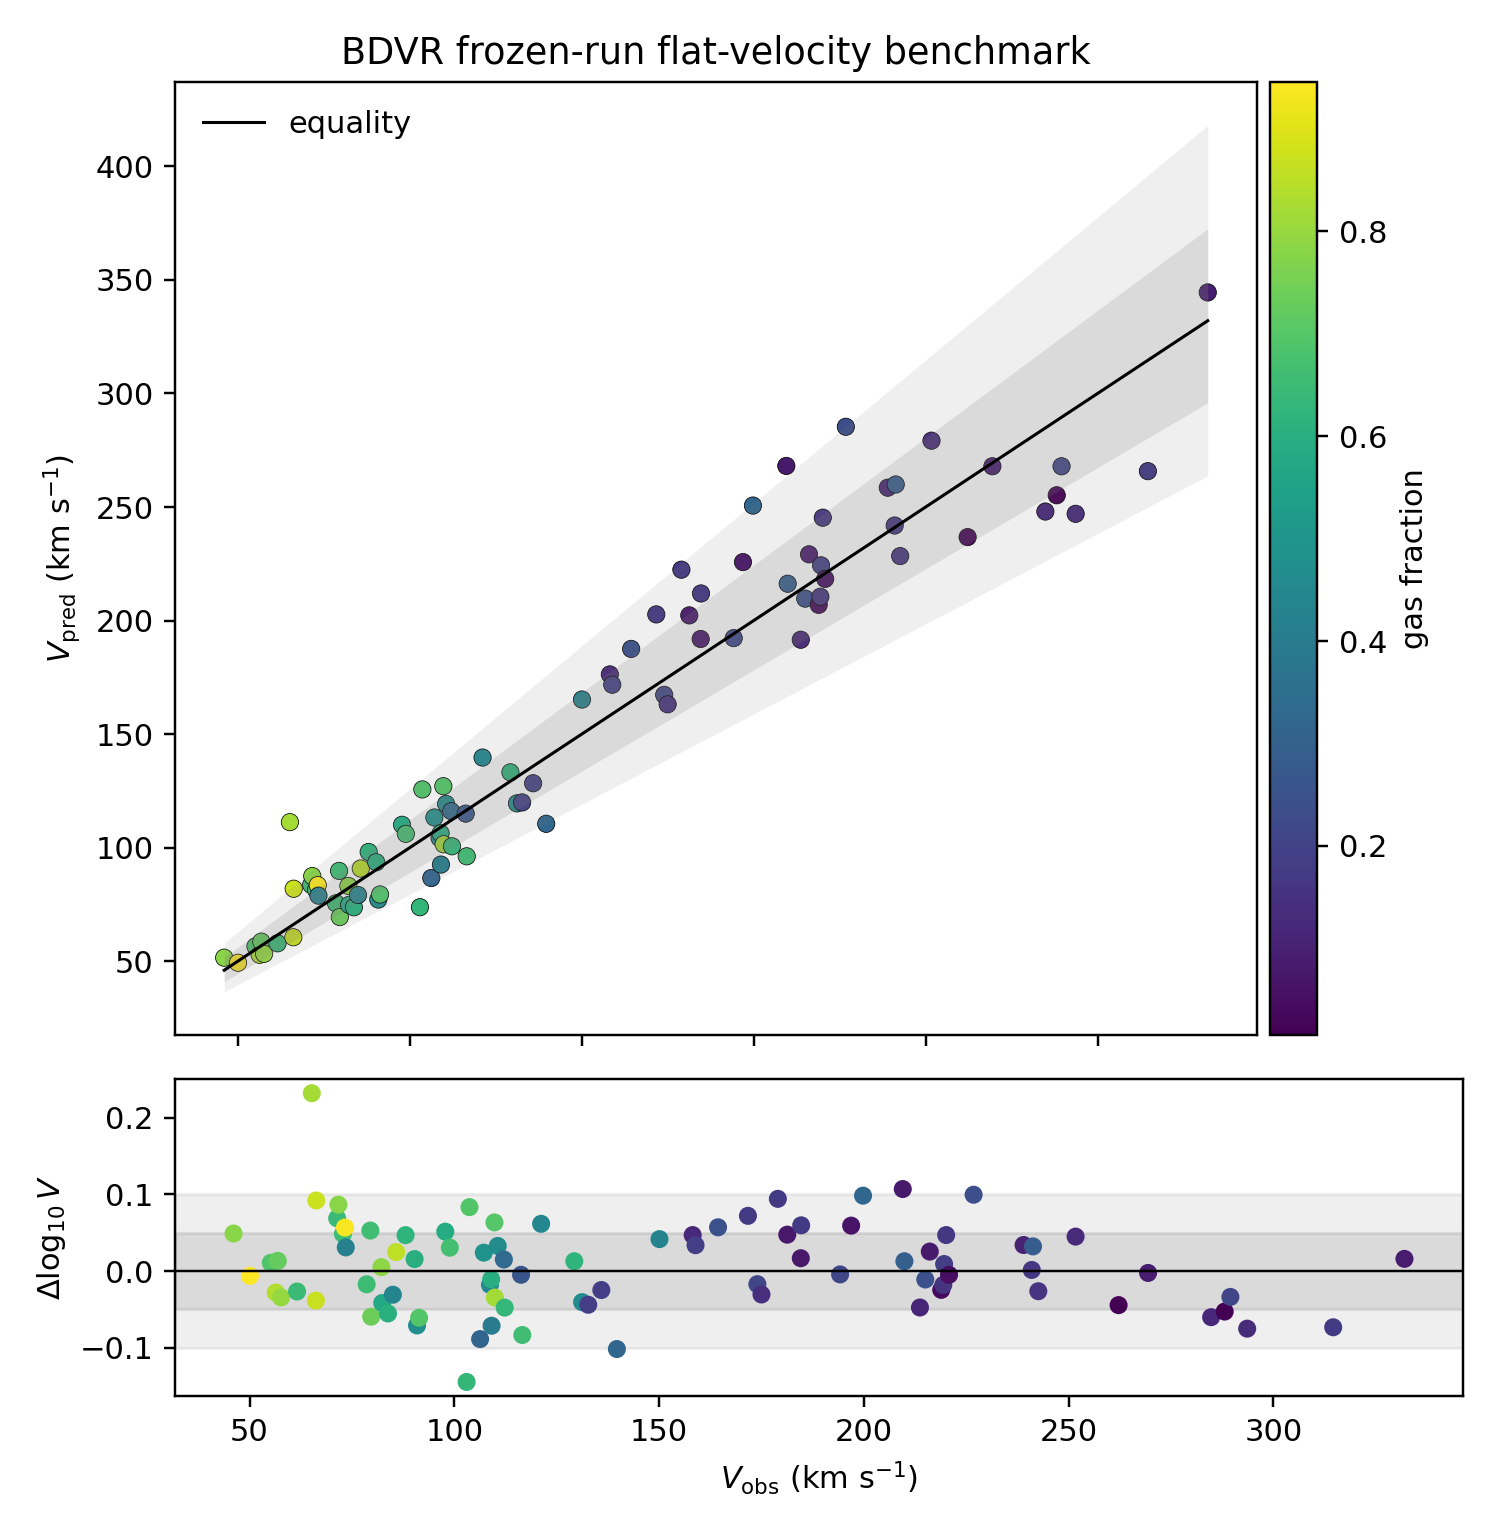
\includegraphics[width=0.9\linewidth]{figures/fig_1_pred_obs_residual_panel.png}
\caption{Predicted versus observed flat velocities for the 87-galaxy SPARC quality-1 evaluation subset. The solid line marks equality; shaded bands indicate $\pm0.05$ and $\pm0.10$ dex. Points are colored by gas fraction. The lower panel shows $\Delta \log_{10} V \equiv \log_{10}(V_{\mathrm{pred}}/V_{\mathrm{obs}})$.}
\label{fig:m5-pred-vs-obs}
\end{figure*}

On the restricted 87-galaxy evaluation subset, the frozen BDVR variant yields a median absolute residual of 0.0416 dex and a mean absolute residual of 0.0457 dex in $\log_{10}(V_{\rm pred}/V_{\rm obs})$, with 83 of 87 galaxies lying within 0.10 dex. Relative to the simple BTFR-like baseline on the same sample, whose median absolute residual is 0.0472 dex, the improvement is modest in descriptive residual units. We therefore interpret the result as suggestive evidence that the added structural terms may carry predictive information, but not yet as decisive evidence for a distinct physical law. Establishing that stronger claim requires uncertainty propagation, resampling tests, and matched comparison to full rotation-curve analyses.

\section{Baseline and ablation comparison}

The baseline comparison evaluates Newtonian baryons, a simple BTFR/MOND-like estimator, scalar-$Q$, halo-only, halo plus star/gas, and full frozen M4c variants on the same sample.

\begin{table*}[t]
\centering
\scriptsize
\caption{Baseline and ablation comparison on the same SPARC quality-1 sample.}
\label{tab:baseline-ablation}
\resizebox{\textwidth}{!}{%
\begin{tabular}{lllllllll}
\toprule
Model & $N$ & Median abs. dex & Mean abs. dex & Max abs. dex & Frac. $<0.10$ & Frac. $<0.15$ & $N>0.20$ & $N>0.30$ \\
\midrule
newtonian\_outer & 87 & 0.249744 & 0.244856 & 0.448825 & 0.0689655 & 0.206897 & 57 & 31 \\
mond\_simple\_btfr & 87 & 0.0472258 & 0.0561134 & 0.205226 & 0.83908 & 0.965517 & 1 & 0 \\
m3\_scalar\_q\_only & 87 & 0.0641311 & 0.0692546 & 0.211354 & 0.758621 & 0.896552 & 1 & 0 \\
m4a\_halo\_only & 87 & 0.0416139 & 0.050371 & 0.23214 & 0.896552 & 0.977011 & 1 & 0 \\
m4b\_halo\_star\_gas & 87 & 0.0404458 & 0.0464392 & 0.23214 & 0.931034 & 0.988506 & 1 & 0 \\
m4c\_full\_frozen & 87 & 0.0416139 & 0.0457214 & 0.23214 & 0.954023 & 0.988506 & 1 & 0 \\
\bottomrule
\end{tabular}%
}
\end{table*}

\begin{figure*}[t]
\centering
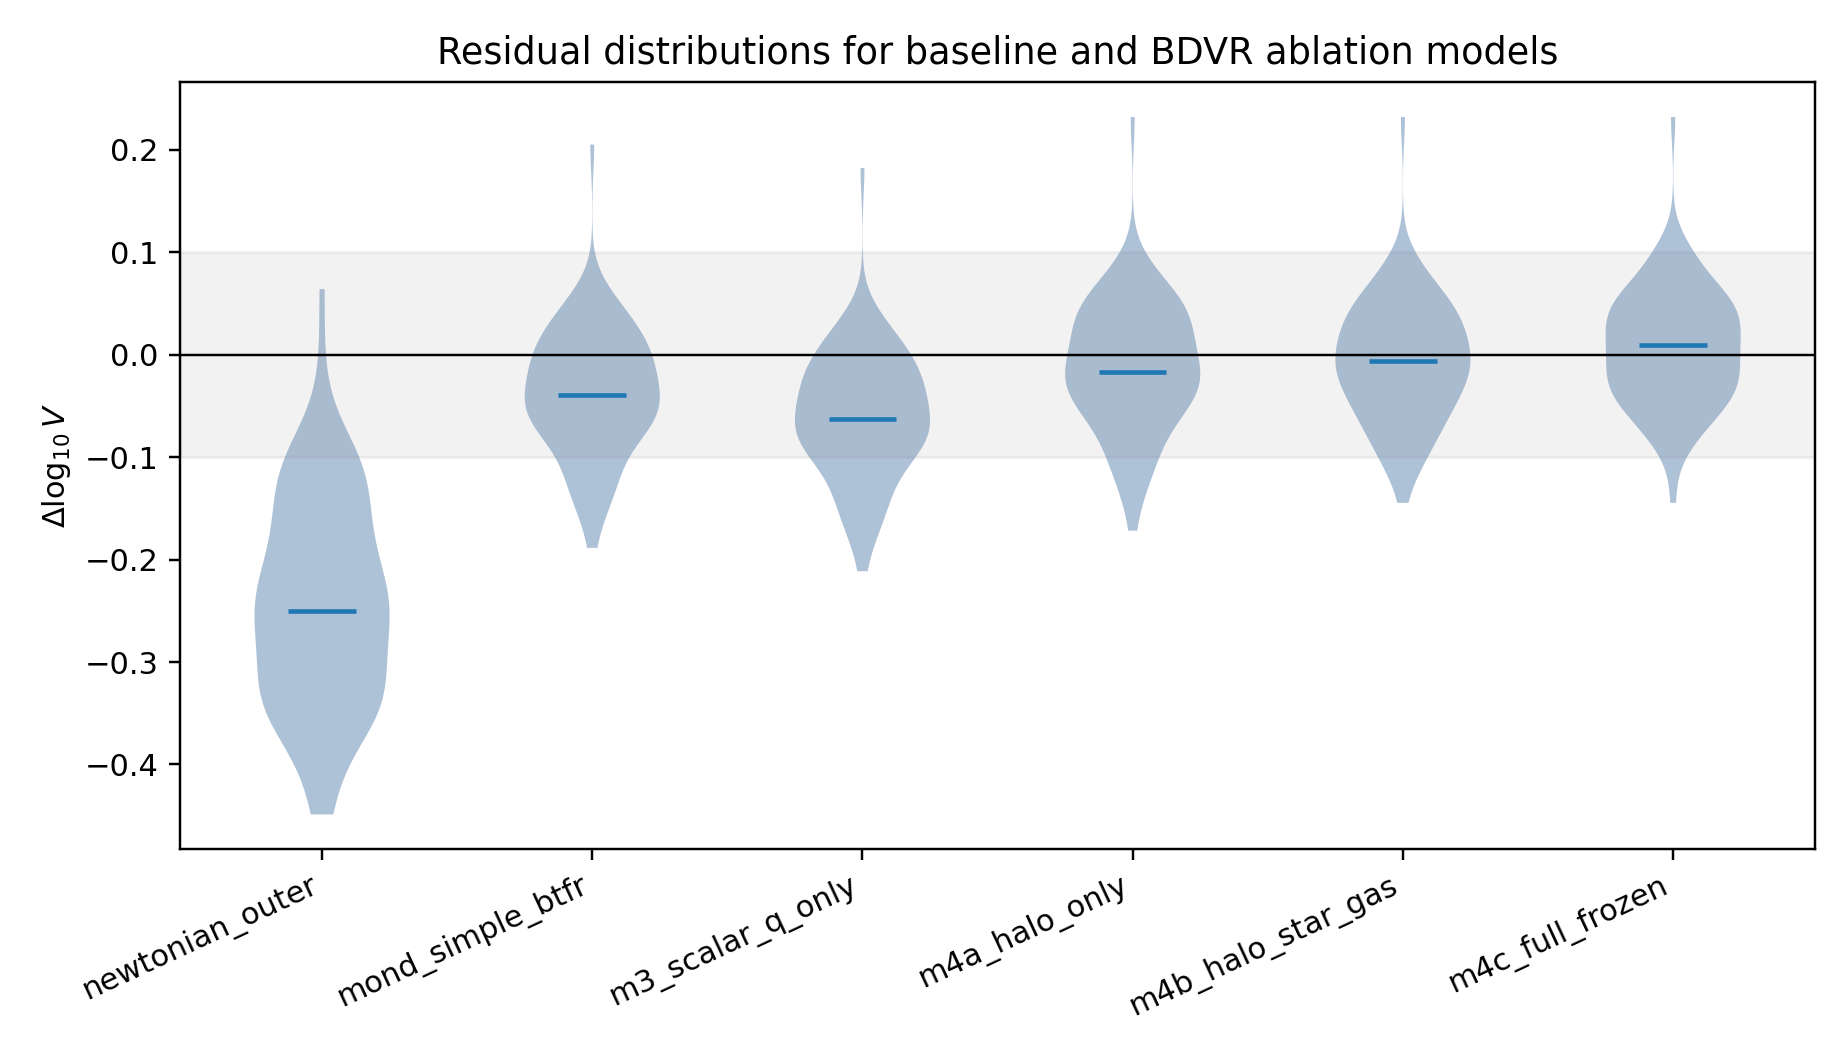
\includegraphics[width=0.9\linewidth]{figures/fig_2_ablation_residual_distributions.png}
\caption{Distribution of per-galaxy log-velocity residuals for the baseline and BDVR ablation models. Violin envelopes show the full residual distributions and median markers; no bootstrap interval is implied in the current descriptive artifact set.}
\label{fig:m5b-residual-distributions}
\end{figure*}

The lowest median absolute residual in this frozen comparison is obtained by \texttt{m4b\_halo\_star\_gas}, with median absolute residual 0.0404 dex. The largest fraction within 0.10 dex is obtained by \texttt{m4c\_full\_frozen}, with 83 of 87 galaxies within 0.10 dex. The ablation table does not identify a unique winner across all scores: m4b yields the lowest median absolute residual, whereas m4c yields the largest fraction within 0.10 dex. We therefore avoid ranking models without a predeclared primary loss function and associated uncertainty intervals. On the present sample, the added radial and structural terms modestly improve selected residual metrics relative to simpler variants, but formal model comparison is still required.


\section{Uncertainty-weighted likelihood comparison}

As a first likelihood-bearing diagnostic, we use the reported SPARC flat-velocity uncertainties and a declared intrinsic floor of 0.030 dex. For each galaxy, the uncertainty entering the Gaussian log-velocity likelihood is $\sigma_{\Delta,i}^2=(e_{V,i}/[\ln(10)V_{\mathrm{flat},i}])^2+\sigma_{\mathrm{floor}}^2$. This calculation is recorded in \texttt{m7\_likelihood\_per\_galaxy.csv}, summarized in \texttt{m7\_model\_likelihood\_summary.csv}, and paired with bootstrap and paired-test outputs in \texttt{m7\_bootstrap\_metric\_intervals.csv} and \texttt{m7\_paired\_model\_tests.csv}.

\begin{table*}[t]
\centering
\scriptsize
\caption{First-pass uncertainty-weighted likelihood diagnostic using reported flat-velocity errors plus a declared intrinsic floor.}
\label{tab:m7-likelihood}
\resizebox{\textwidth}{!}{%
\begin{tabular}{llllllll}
\toprule
Model & $N$ & $\ln\mathcal{L}$ & $k$ & AIC & BIC & $\Delta$AIC & $\Delta$BIC \\
\midrule
m4c\_full\_frozen & 87 & 89.6503 & 5 & -169.301 & -156.971 & 0 & 0 \\
m4b\_halo\_star\_gas & 87 & 81.0501 & 4 & -154.1 & -144.237 & 15.2005 & 12.7346 \\
m4a\_halo\_only & 87 & 60.4978 & 3 & -114.996 & -107.598 & 54.3051 & 49.3732 \\
mond\_simple\_btfr & 87 & 23.4547 & 1 & -44.9095 & -42.4436 & 124.391 & 114.528 \\
m3\_scalar\_q\_only & 87 & -54.5169 & 1 & 111.034 & 113.5 & 280.334 & 270.471 \\
newtonian\_outer & 87 & -2120.98 & 0 & 4241.97 & 4241.97 & 4411.27 & 4398.94 \\
\bottomrule
\end{tabular}%
}
\end{table*}

The table reports AIC and BIC under an explicit parameter-count policy for frozen predictors. Because distance, inclination, stellar mass-to-light, H I mass, covariance terms, and full rotation-curve information are not yet propagated, this likelihood comparison is an intermediate audit statistic rather than a final model-selection result. WAIC, LOO, and Bayes factors are not claimed here because no hierarchical posterior model has yet been implemented.

\begin{figure*}[t]
\centering
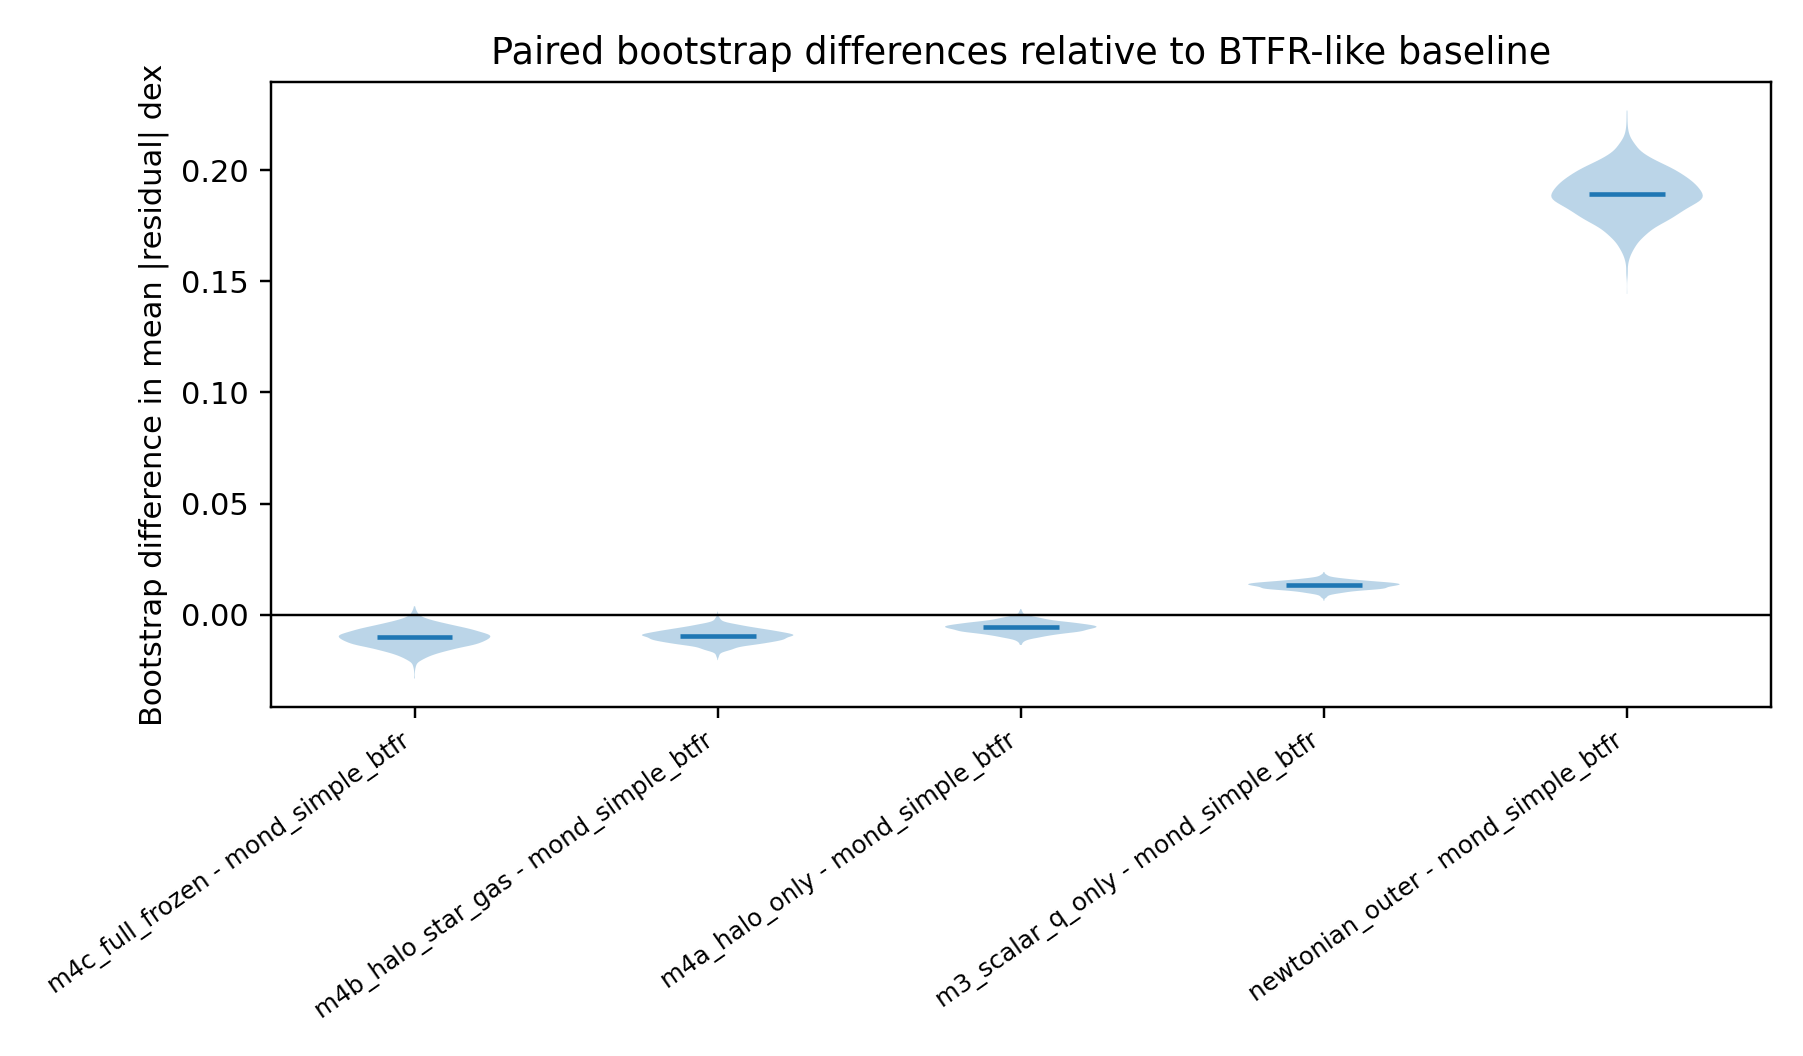
\includegraphics[width=0.9\linewidth]{figures/fig_m7_bootstrap_model_differences.png}
\caption{Paired bootstrap differences in mean absolute log-velocity residual relative to the BTFR-like baseline. The figure is a first-pass audit diagnostic using the fixed residual vectors and does not include full observational covariance propagation.}
\label{fig:m7-bootstrap-differences}
\end{figure*}


\section{Residual structure and retained verification target}

\begin{table*}[t]
\centering
\scriptsize
\caption{Largest residual correlations by model class. These diagnostics are used to characterize residual structure, not as additional tuning inputs.}
\label{tab:residual-correlations}
\resizebox{\textwidth}{!}{%
\begin{tabular}{llllll}
\toprule
Model & Variable & $N$ & Pearson $r$ & Spearman $\rho$ & Slope \\
\midrule
m3\_scalar\_q\_only & stellar\_to\_gas\_ratio & 87 & -0.418072 & -0.377069 & -0.00275418 \\
m3\_scalar\_q\_only & star\_frac & 87 & -0.386556 & -0.377069 & -0.0872545 \\
m3\_scalar\_q\_only & gas\_frac & 87 & 0.386556 & 0.377069 & 0.0872545 \\
m3\_scalar\_q\_only & v\_flat\_obs\_km\_s & 87 & -0.421025 & -0.376996 & -3.5407e-04 \\
m3\_scalar\_q\_only & S\_star\_gas & 87 & -0.395256 & -0.373298 & -0.394874 \\
m4a\_halo\_only & S\_star\_gas & 87 & -0.424908 & -0.380006 & -0.433895 \\
m4a\_halo\_only & stellar\_to\_gas\_ratio & 87 & -0.444008 & -0.367427 & -0.0029898 \\
m4a\_halo\_only & star\_frac & 87 & -0.383092 & -0.367427 & -0.0883871 \\
m4a\_halo\_only & gas\_frac & 87 & 0.383092 & 0.367427 & 0.0883871 \\
m4a\_halo\_only & v\_flat\_obs\_km\_s & 87 & -0.412096 & -0.359244 & -3.5424e-04 \\
m4b\_halo\_star\_gas & v\_flat\_obs\_km\_s & 87 & -0.336134 & -0.305406 & -2.7025e-04 \\
m4b\_halo\_star\_gas & star\_frac & 87 & -0.300895 & -0.283626 & -0.0649334 \\
m4b\_halo\_star\_gas & gas\_frac & 87 & 0.300895 & 0.283626 & 0.0649334 \\
m4b\_halo\_star\_gas & stellar\_to\_gas\_ratio & 87 & -0.283907 & -0.283626 & -0.00178812 \\
m4b\_halo\_star\_gas & S\_star\_gas & 87 & -0.250682 & -0.264977 & -0.239431 \\
m4c\_full\_frozen & M\_gas\_Msun & 87 & 0.187678 & 0.330177 & 9.8263e-13 \\
m4c\_full\_frozen & $R_{\rm H\,I}$ & 87 & 0.226596 & 0.319846 & 8.7464e-04 \\
m4c\_full\_frozen & H\_halo & 87 & 0.196081 & 0.202687 & 0.24409 \\
\bottomrule
\end{tabular}%
}
\end{table*}

\begin{figure*}[t]
\centering
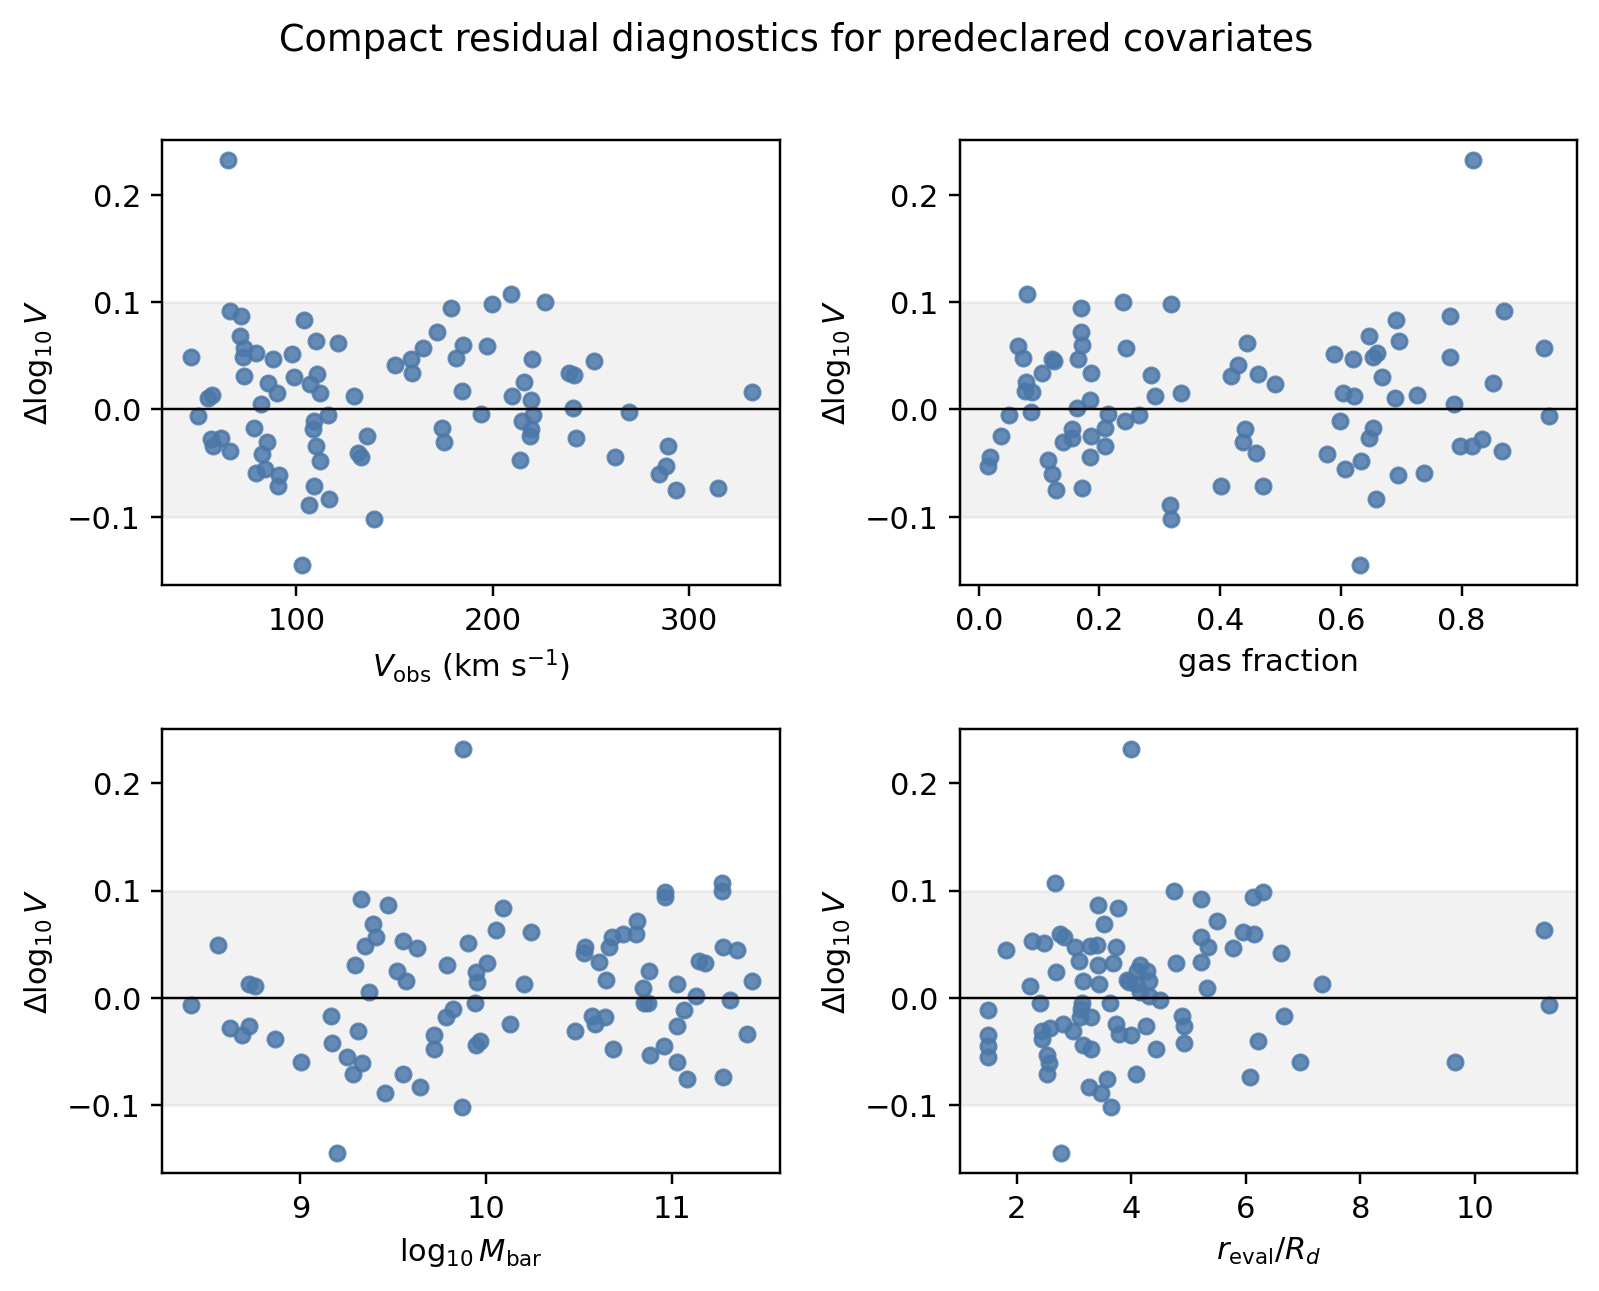
\includegraphics[width=0.9\linewidth]{figures/fig_3_residual_covariates_compact.png}
\caption{Residual diagnostics for the frozen BDVR benchmark. Panels show $\Delta\log_{10}V$ against predeclared covariates only; broader exploratory diagnostics are retained as machine-readable artifacts rather than promoted to primary inference.}
\label{fig:residual-dashboard}
\end{figure*}

The residual-correlation diagnostics are exploratory structure tests rather than tuning inputs or formal multiple-comparison results. UGC07125 is retained in all metrics and is not tuned away. For UGC07125, the M5d inversion gives $M_{\rm part,req}=8.8558e+08M_\odot$, compared with catalogued $M_b=7.5126e+09M_\odot$ and $M_*=1.3560e+09M_\odot$. The required participating fraction is 0.1179. Because the required participating mass is smaller than the catalogued stellar mass alone, the implied gas participation is a negative required gas participation; this is a diagnostic breakdown or systematics flag, not a physically meaningful gas-participation estimate. This object is interpreted as a verification target rather than a resolved case.

The appropriate next checks are external: resolved H~I kinematics, inclination and warp reliability, approaching/receding asymmetry, gas surface-density structure, and mass-estimate systematics.

\section{Discussion}

The present evidence is consistent with interpreting BDVR as an empirical reparameterization of the baryon--velocity relation rather than as direct evidence for a new microscopic mechanism. The radial and structural modifiers may be capturing population trends already present in the SPARC sample, such as the dependence of $V_{\rm flat}$ on gas content, morphology, or the radius at which the flat part of the curve is measured. Distinguishing a genuinely new physical law from an efficient empirical fit will require full rotation-curve tests, hierarchical treatment of observational systematics, and evaluation on larger, more homogeneous data sets.

A remaining interpretive limitation is that the $V_{\rm flat}$ estimator depends on the product $Q_{\mathrm{eff}}^2 a_0$, so the present benchmark does not sharply distinguish a preferred acceleration scale from a preferred response normalization. We have separated the measurement-domain clock variable $\mathcal{T}$ from the morphology index $T_{\mathrm{morph}}$ to avoid implying a deeper connection between those quantities than is demonstrated here.

As a reservoir-mediated stabilization interpretation, enhanced rotation support may help extended baryonic disks remain dynamically cold, resist premature central collapse, and regulate star formation by keeping gas distributed over long dynamical times. This is the bounded ``why'' version of the argument: rotationally supported disks are stabilized by orbital support and multi-component disk stability, while gas surface density and feedback regulate star formation \cite{Toomre1964,Kennicutt1998,Bigiel2008,Leroy2008,Ostriker2011}. Disk formation models likewise tie long-lived disks to angular momentum, surface density, and halo/disk structure \cite{FallEfstathiou1980,MoMaoWhite1998,Dalcanton1997,RomeoMogotsi2017}. In BDVR language this suggests that the response term, if physical, may act as a governor for mature disk survival rather than merely as a curve-fitting correction.

The juvenile-to-mature hypothesis is more speculative. It treats UGC07125-like residuals as possible signs that reservoir coupling is conditional: gas-rich, diffuse, or dynamically unsettled systems may not activate the full response, whereas organized stellar disks may. We include this as a supplementary interpretation rather than as evidence already established by the flat-velocity residuals. The current paper does not fit a governor surface, but it motivates future tests in which an activation factor $A_{\rm gov}$ is inferred against stellar fraction, gas fraction, surface density, and settling diagnostics.

The stabilization and maturation interpretations are motivated by established ideas about disk stability, gas consumption, and angular-momentum-supported disk formation, but they remain heuristic until tested against full rotation curves and independent settling diagnostics \cite{Toomre1964,Kennicutt1998,Bigiel2008,Leroy2008,Ostriker2011,FallEfstathiou1980,MoMaoWhite1998,Dalcanton1997}.

The main theoretical task is to derive $Q_0$, $H$, $S_{\rm sg}$, $S_{\rm int}$, and $a_0$ from deeper bound-domain current variables rather than treating them as effective phenomenological factors. The main observational task is uncertainty-aware comparison to BTFR/RAR and halo-model baselines, followed by external tests of retained failure modes such as UGC07125 with resolved H I and baryonic-participation diagnostics.

\section{Conclusions}

BDVR should presently be regarded as a falsifiable phenomenological ansatz for predicting $V_{\rm flat}$ in a restricted SPARC subset. Its current success is limited to that frozen-run benchmark and does not yet establish a fundamental theory or a cosmological framework. It is not a complete replacement for dark matter. A decisive test of BDVR now requires a public, uncertainty-aware comparison to BTFR/RAR and halo-model baselines on the same galaxies, followed by external prediction on independent data. The immediate next tests are: analysis of full SPARC rotation curves rather than only $V_{\rm flat}$; external evaluation on independent H I data sets and forthcoming large SPARC-like products; and resolved H I follow-up of persistent outliers such as UGC07125.

\clearpage
\FloatBarrier
\appendix

\section{UGC07125 as a retained diagnostic target}

UGC07125 is retained as a systematics and follow-up target, not as a solved physical estimate. The table and figures below document why the object remains useful: it is the leading retained residual, the participating-mass inversion produces a negative required gas-participation diagnostic, and resolved H I or inclination/asymmetry checks are needed before any physical interpretation is assigned.

\begin{table*}[t]
\centering
\scriptsize
\caption{UGC07125 retained-outlier audit fields and participating-mass diagnostic quantities.}
\label{tab:ugc07125}
\resizebox{\textwidth}{!}{%
\begin{tabular}{lll}
\toprule
Field & Value & Source \\
\midrule
galaxy\_name & UGC07125 & m5\_prediction \\
T & 9.0 & m5\_prediction \\
v\_flat\_obs\_km\_s & 65.2 & m5\_prediction \\
v\_m5\_bdvr\_km\_s & 111.27246923349932 & m5\_prediction \\
velocity\_ratio\_pred\_over\_obs & 1.7066329637039772 & m5\_prediction \\
log10\_velocity\_error & 0.2321401297980161 & m5\_prediction \\
abs\_log10\_velocity\_error & 0.2321401297980161 & m5\_prediction \\
M\_baryon\_Msun & 7512569999.999999 & m5\_prediction \\
M\_star\_Msun & 1356000000.0 & m5\_prediction \\
M\_gas\_Msun & 6156569999.999999 & m5\_prediction \\
star\_frac & 0.1804974862131068 & m5\_prediction \\
gas\_frac & 0.8195025137868931 & m5\_prediction \\
stellar\_to\_gas\_ratio & 0.2202525107324371 & m5\_prediction \\
Rdisk & 3.38 & m5\_prediction \\
$R_{\rm H\,I}$ & 23.04 & m5\_prediction \\
$R_{\rm H\,I}/R_d$ & 6.816568047337278 & m5d\_participation \\
Q\_eff & 1.13195243693273 & m5\_prediction \\
H\_halo & 1.2573763420608173 & m5\_prediction \\
S\_star\_gas & 1.0 & m5\_prediction \\
S\_internal & 1.0 & m5\_prediction \\
S\_struct & 1.0 & m5\_prediction \\
M\_part\_required\_Msun & 885580433.570339 & m5d\_participation \\
participation\_fraction\_required & 0.11787982455675476 & m5d\_participation \\
gas\_participation\_required & -0.0764093588523579 & m5d\_participation \\
gas\_participation\_required\_status & stellar\_mass\_alone\_exceeds\_required\_participating\_mass & m5d\_participation \\
\bottomrule
\end{tabular}%
}
\end{table*}

\begin{figure*}[p]
\centering
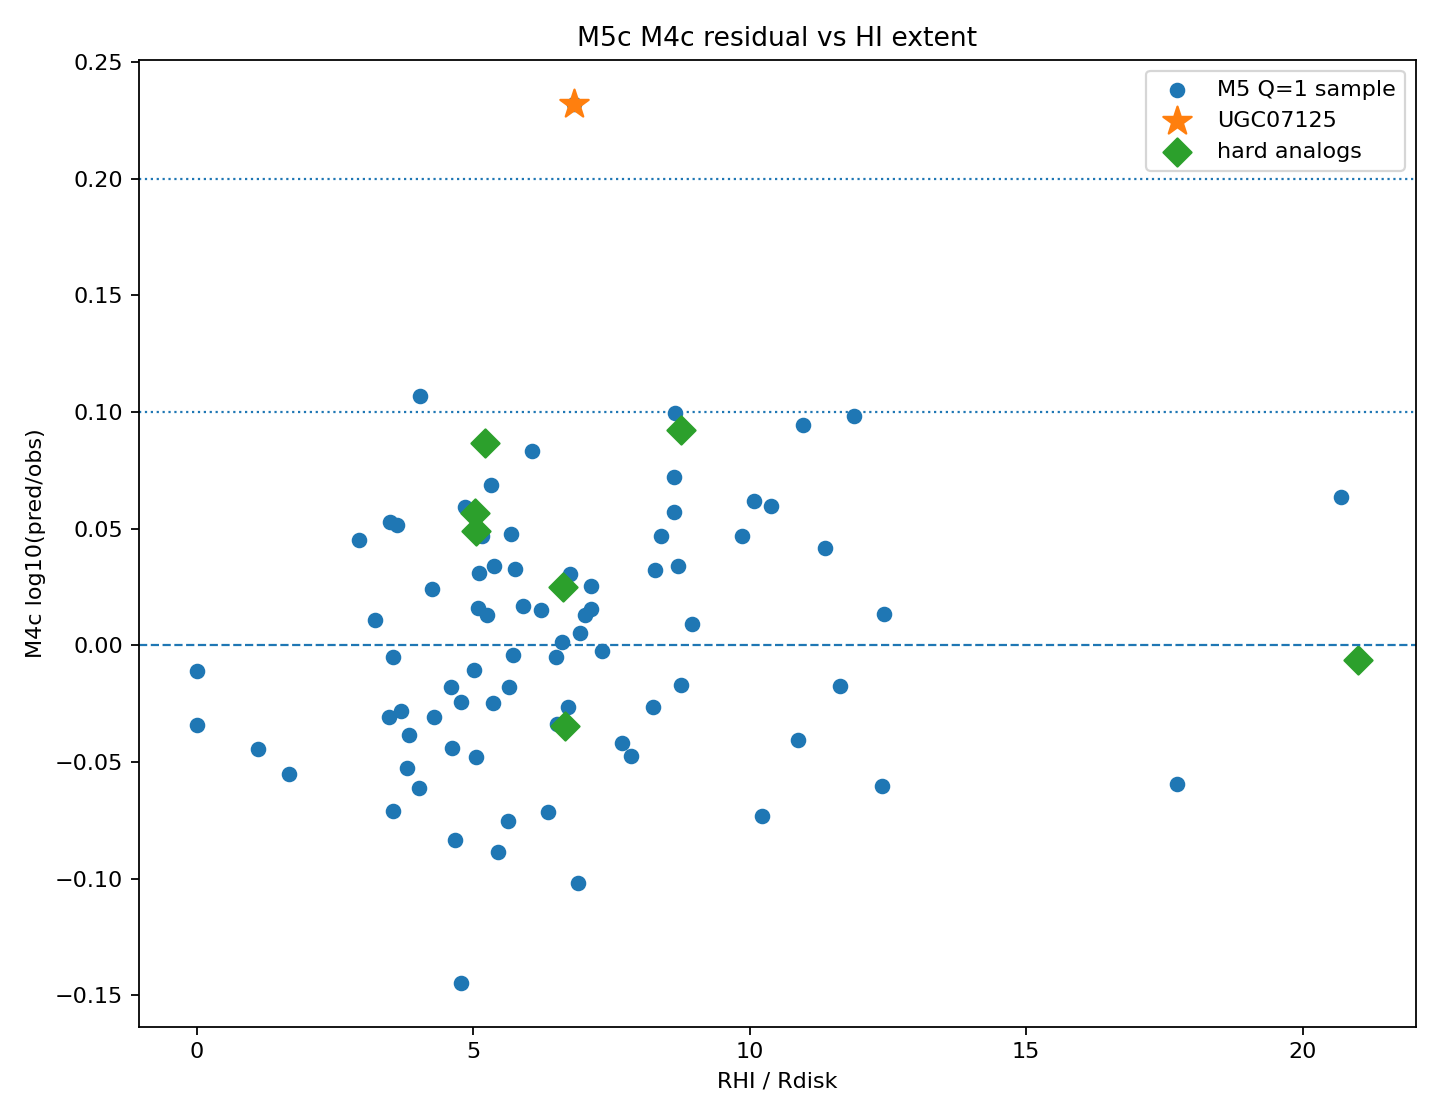
\includegraphics[width=0.9\linewidth]{figures/appendix_fig_ugc07125_hi_extent.png}
\caption{UGC07125 analog-search residual behavior versus H~I extent.}
\label{fig:ugc-hi-extent}
\end{figure*}

\FloatBarrier

\begin{figure*}[p]
\centering
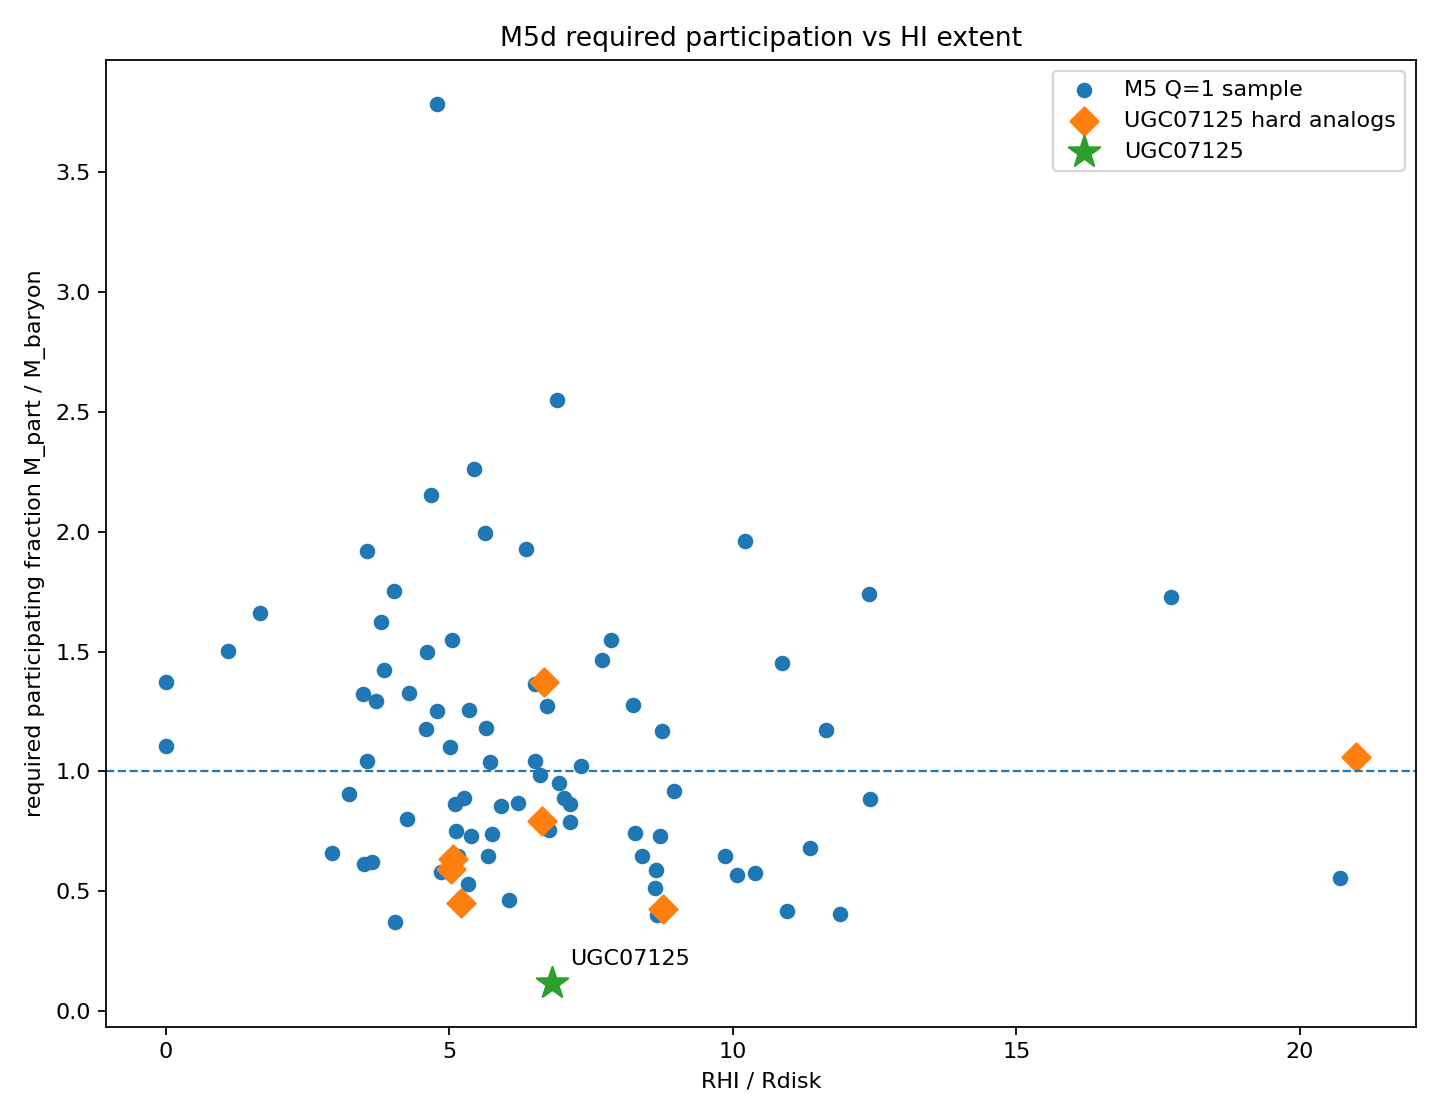
\includegraphics[width=0.9\linewidth]{figures/appendix_fig_ugc07125_participation_vs_rhi.png}
\caption{Required participating mass fraction versus H~I extent in the M5d inversion diagnostic.}
\label{fig:ugc-participation-rhi}
\end{figure*}

\FloatBarrier


\clearpage
\FloatBarrier
\section{87-galaxy evaluation subset}

The complete machine-readable 87-galaxy table is included in the accompanying CSV archive. It lists the galaxy name, SPARC quality flag, $T_{\mathrm{morph}}$, $V_{\mathrm{flat}}$, $e_{V_{\mathrm{flat}}}$, luminosity, H~I mass, disk scale, H~I radius, distance, inclination, SPARC reference codes, constructed stellar/gas/baryonic masses, $r_{\mathrm{eval}}/R_d$, and the selection rule. The complete 87-galaxy evaluation subset is provided as machine-readable Table S1 and in the accompanying CSV archive; we therefore do not reproduce the full galaxy-name list inline. For a visual sample-identity audit only, Table~\ref{tab:evaluation-subset-names} gives the names in a compact table.


\begin{table*}[p]
\centering
\scriptsize
\caption{Evaluation subset galaxy names. This compact table is included only for visual audit of the sample identity; the authoritative subset with columns and selection flags is the machine-readable CSV.}
\label{tab:evaluation-subset-names}
\begin{tabular}{llll}
\toprule
Galaxy & Galaxy & Galaxy & Galaxy \\
\midrule
D631-7 & DDO064 & DDO161 & ESO079-G014 \\
ESO116-G012 & ESO563-G021 & F563-1 & F563-V2 \\
F568-V1 & F571-8 & F574-1 & F579-V1 \\
F583-1 & IC4202 & NGC0024 & NGC0100 \\
NGC0801 & NGC0891 & NGC1003 & NGC1090 \\
NGC2403 & NGC2841 & NGC2903 & NGC2998 \\
NGC3109 & NGC3198 & NGC3521 & NGC3741 \\
NGC3893 & NGC3917 & NGC3953 & NGC3972 \\
NGC3992 & NGC4088 & NGC4100 & NGC4157 \\
NGC4183 & NGC4217 & NGC4559 & NGC5005 \\
NGC5033 & NGC5055 & NGC5371 & NGC5585 \\
NGC5907 & NGC5985 & NGC6195 & NGC6503 \\
NGC6674 & NGC6946 & NGC7331 & NGC7814 \\
UGC00128 & UGC00731 & UGC01230 & UGC01281 \\
UGC02487 & UGC02885 & UGC03205 & UGC03546 \\
UGC04278 & UGC04325 & UGC04499 & UGC05005 \\
UGC05721 & UGC06399 & UGC06446 & UGC06614 \\
UGC06667 & UGC06786 & UGC06917 & UGC06930 \\
UGC06983 & UGC07125 & UGC07151 & UGC07399 \\
UGC07524 & UGC07603 & UGC08286 & UGC08490 \\
UGC08550 & UGC09133 & UGC10310 & UGC11455 \\
UGC11914 & UGC12632 & UGCA442 &  \\
\bottomrule
\end{tabular}
\end{table*}

\FloatBarrier



\clearpage
\FloatBarrier
\section{Freeze chronology and audit manifest}

The freeze chronology remains partly unresolved. The current evidence package documents the frozen numerical artifacts used for this draft and documents that no per-galaxy response refitting is applied during the present evaluation, but the complete historical tuning chronology is not established by current artifacts. The audit manifest files \texttt{cghstc34\_audit\_manifest.csv} and \texttt{cghstc34\_audit\_manifest.json} list the CSV, figure, manuscript, bibliography, likelihood, and bootstrap artifacts required to reproduce the audit trail.

\begin{table*}[t]
\centering
\scriptsize
\caption{Freeze-chronology status for the current evidence package.}
\label{tab:freeze-chronology}
\resizebox{\textwidth}{!}{%
\begin{tabular}{lll}
\toprule
item & status & evidence \\
\midrule
M4c/M5 numeric artifact freeze & documented for this evidence bundle & m6\_source\_artifacts\_manifest.json records upstream file paths, sizes, and hashes \\
No per-galaxy response refitting in generated M4c evaluation & documented for this run & global parameter table and per-galaxy residual outputs \\
Complete historical tuning chronology before the frozen run & not established by current artifacts & manuscript must use evaluation/frozen-run benchmark language rather than stronger claims \\
Uncertainty propagation and formal model comparison & not implemented in current artifacts & listed as decisive future work, not claimed as current evidence \\
\bottomrule
\end{tabular}%
}
\end{table*}


\clearpage
\FloatBarrier
\section{Possible stabilization interpretation of enhanced rotational support}

We use ``enhanced rotation support'' here in a dynamical, not teleological, sense. The relevant physical question is whether an additional effective support term changes which baryonic disk configurations remain long-lived. A cold disk must balance self-gravity, orbital support, pressure/turbulent support, and feedback. In the standard disk-stability language, rotation and epicyclic support enter the stability threshold, while gas surface density controls both gravitational instability and star-formation efficiency \cite{Toomre1964,Kennicutt1998,Bigiel2008,Leroy2008,RomeoMogotsi2017}. Thus enhanced rotation support may help extended baryonic disks remain dynamically cold without rapidly collapsing into compact stellar systems.

The BDVR interpretation of this fact is intentionally modest. If the response term is more than an empirical reparameterization, its possible evolutionary role would be to keep gas and stars in broad, rotating orbits, thereby slowing premature baryonic collapse and allowing star formation to proceed over long depletion times. Feedback-regulated disk models already treat star formation as a self-regulated process involving gas weight, turbulence, and stellar feedback \cite{Ostriker2011}. BDVR does not replace those mechanisms in the present work; it only motivates the future question of whether the inferred response amplitude correlates with the same disk-stability and gas-regulation variables.

\clearpage
\FloatBarrier
\section{Juvenile-to-mature reservoir activation hypothesis}

Appendix E is a hypothesis-generating supplement, not a fitted extension of the present benchmark. We use it to define an observationally testable governor variable $A_{\rm gov}$ that may depend on stellar fraction, gas fraction, surface density, and settling diagnostics. No transition surface is inferred in the present work. The candidate galactic maturation threshold remains an interpretive extension: in this hypothesis, a juvenile system is gas-rich, diffuse, or dynamically unsettled, and uses baryons primarily to build stellar structure. A mature system has enough organized stellar and gas disk structure to couple efficiently to the reservoir-like response. A minimal future governor extension would write
\begin{equation}
v_{\rm BDVR}^2 = v_N^2 + A_{\rm gov} Q_{\rm eff} v_{\rm res}^2,
\qquad 0\le A_{\rm gov}\le 1,
\end{equation}
where $A_{\rm gov}\simeq0$ denotes suppressed coupling and $A_{\rm gov}\simeq1$ denotes full coupling.

The natural empirical variables are stellar fraction $f_*=M_*/M_{\rm bar}$, gas fraction $f_{\rm gas}=M_g/M_{\rm bar}$, baryonic surface-density or surface-brightness proxies, and settling diagnostics such as H I asymmetry, warps, or approaching/receding mismatch. Disk-formation theory already links mature disks to angular momentum retention, surface density, and halo/disk structure \cite{FallEfstathiou1980,MoMaoWhite1998,Dalcanton1997}. In the present artifact set we do not fit $A_{\rm gov}$ or claim a discovered transition surface. We only show residual diagnostics against available maturity proxies in Fig.~\ref{fig:maturity-residual-diagnostics} as a way to define the next test.

\begin{figure*}[p]
\centering
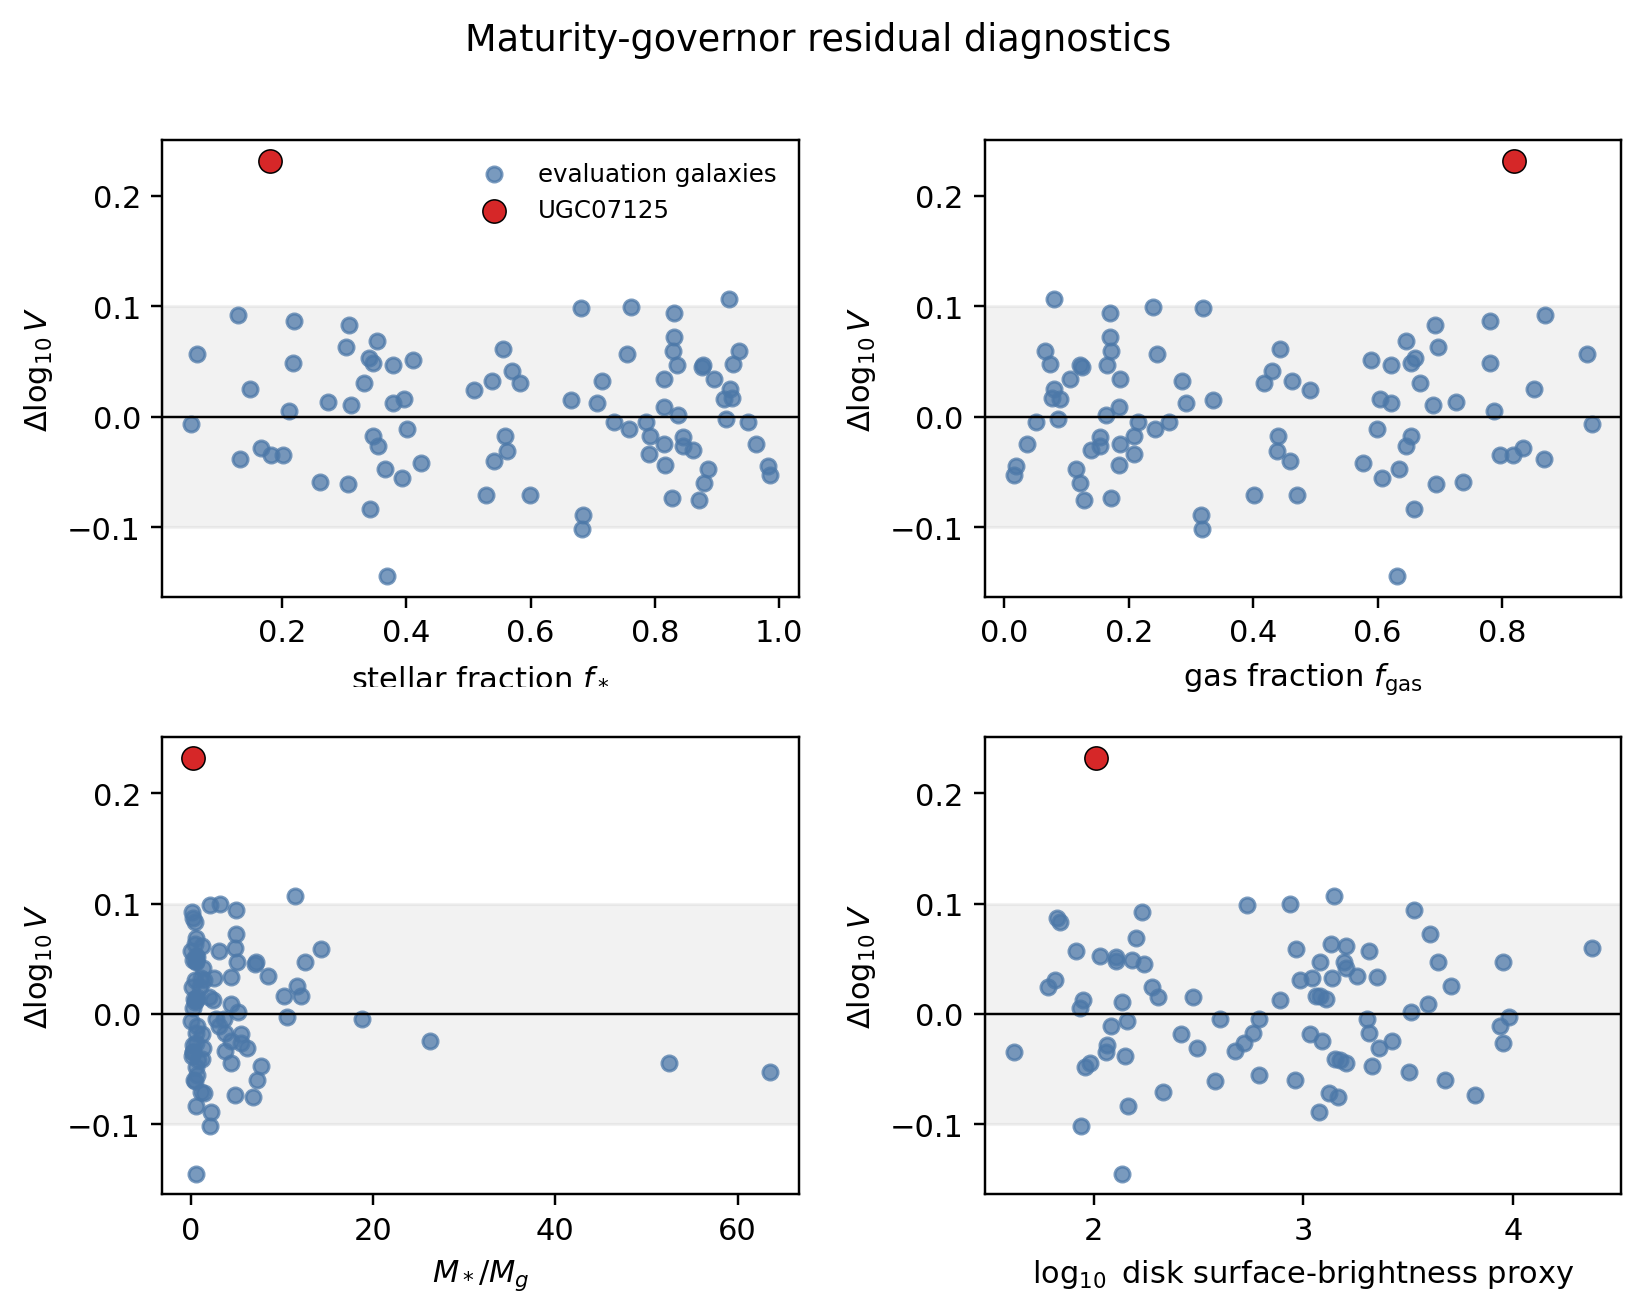
\includegraphics[width=0.9\linewidth]{figures/appendix_fig_maturity_residual_diagnostics.png}
\caption{Maturity-governor residual diagnostics for the frozen BDVR benchmark. Panels show log-velocity residuals against stellar fraction, gas fraction, stellar-to-gas ratio, and a disk surface-brightness proxy. UGC07125 is highlighted because it is the leading retained residual; the figure is diagnostic only and does not fit a governor surface.}
\label{fig:maturity-residual-diagnostics}
\end{figure*}

\FloatBarrier

If the hypothesis is useful, UGC07125 should not be unique: the same pattern should recur in gas-rich, diffuse, or dynamically unsettled systems where the full BDVR response overpredicts $V_{\rm flat}$. The falsifiable next step is therefore not to retune the current M4c law, but to infer or constrain $A_{\rm gov}$ on held-out galaxies and test whether the inferred activation rises across a galactic maturation threshold.

\section{Reproducibility and availability}

The numerical tables in this manuscript are generated from the CGHSTC-34 artifact records under \texttt{runs/cghstc\_34\_m6\_paper\_artifacts/} in the project tree. The source manifest \texttt{m6\_source\_artifacts\_manifest.json} records the upstream tables and figures used for this draft. A submission candidate should archive the exact source tree, the SPARC-derived input policy, the generated tables, and the figure files referenced in this document.

\clearpage
\FloatBarrier
\nocite{*}
\bibliographystyle{apsrev4-2}
\bibliography{refs_stub}

\end{document}
